\newgeometry{left=0mm, right=0mm, top=0mm, bottom=0mm} 
% Remove header/footer elements for a clean look
\pagestyle{empty}

% Insert the image stretched to the paper dimensions
\noindent 
% TITLE PAGE and COPTYRIGHT
\begin{center}
	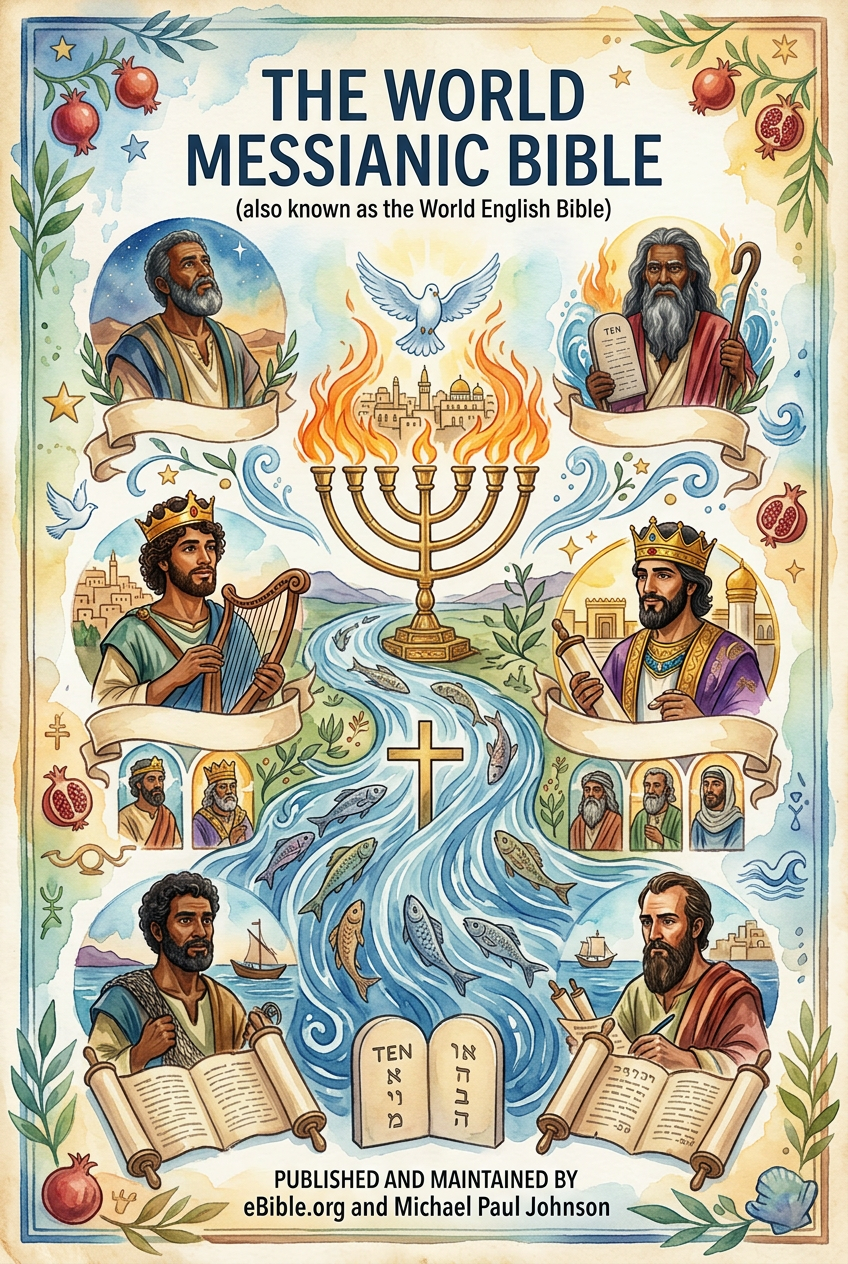
\includegraphics[width=\paperwidth, height=\paperheight]{images/title-page.png}
	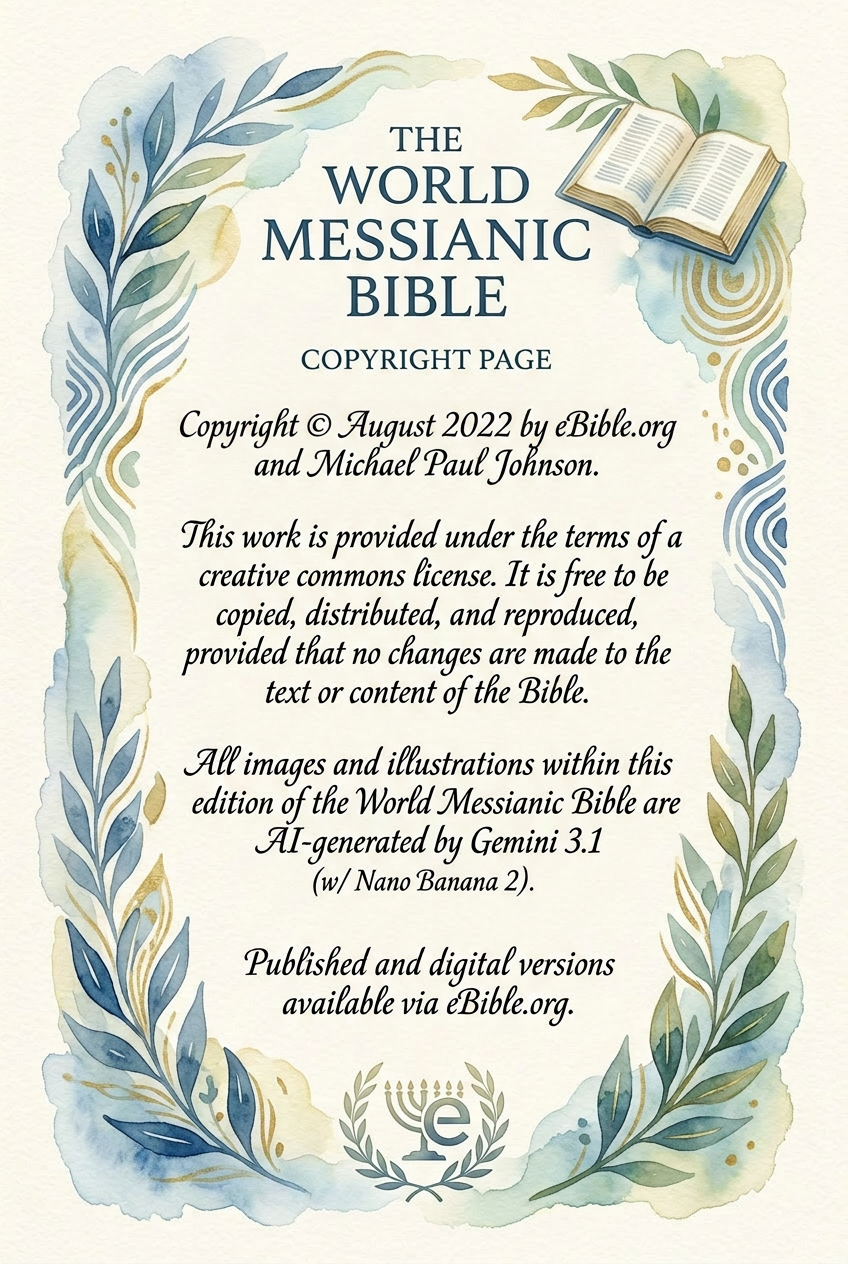
\includegraphics[width=\paperwidth, height=\paperheight]{images/copyright.png}
	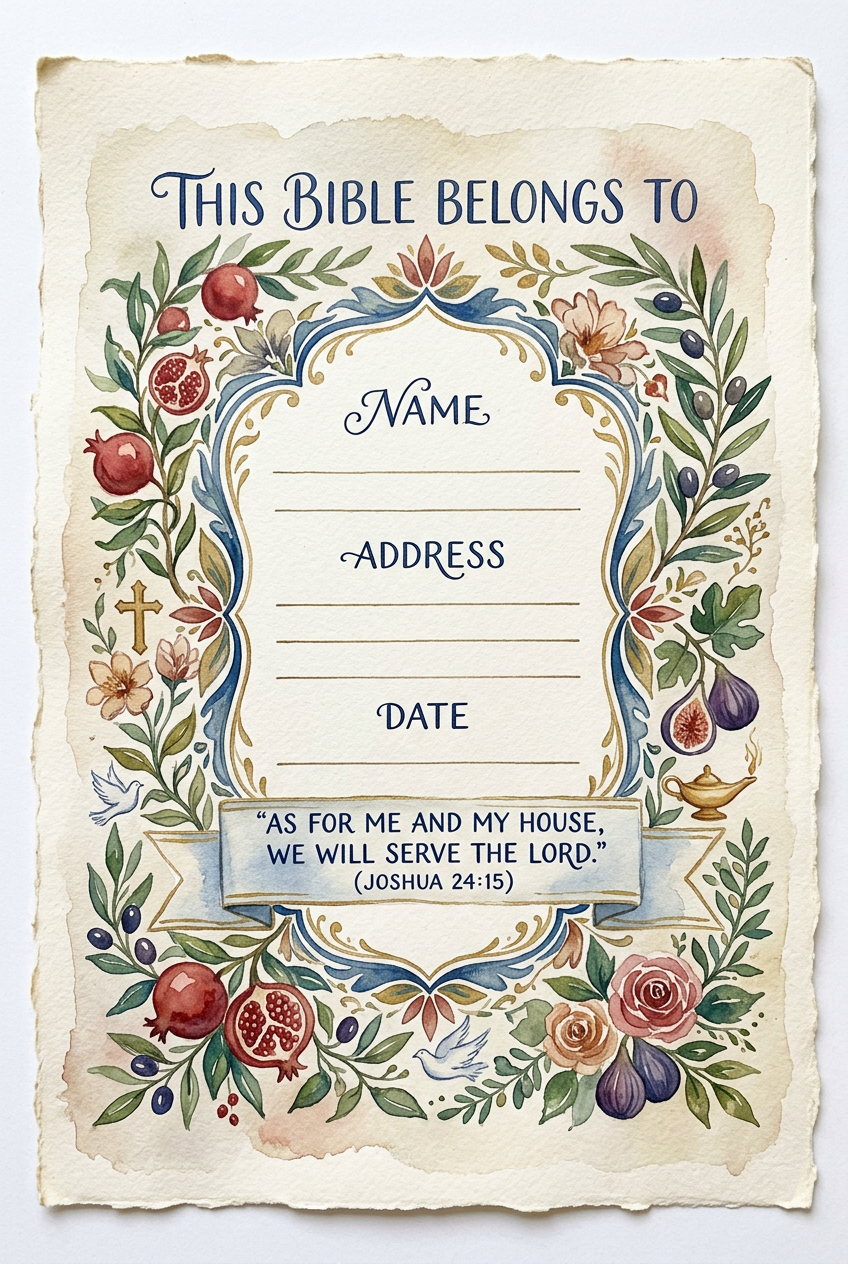
\includegraphics[width=\paperwidth, height=\paperheight]{images/bookplate.png}
	\clearpage
	\clearpage
\end{center}

% TOC and INTRODUCTION
\newgeometry{	inner=20mm,  % Margin closest to the binding
	outer=20mm,  % Margin on the outside edge (allows for journaling space)
	top=20mm,
	bottom=20mm} 

\tableofcontents
\markboth{Contents}{Contents} 

\addcontentsline{toc}{chapter}{Disclaimers}
\chapter*{Disclaimers}\markboth{Disclaimers}{Disclaimers} 
\vspace{-1in}

\par\textbf{Original Copyright Statement}

According to \href{https://ebible.org/engwmb/copyright.htm}{eBible.org}:
\begin{quotation}
	
 The World Messianic Bible is not copyrighted, however "World Messianic Bible" is a Trademark.
 
You may copy, publish, proclaim, distribute, redistribute, sell, give away, quote, memorize, read publicly, broadcast, transmit, share, back up, post on the Internet, print, reproduce, preach, teach from, and use the World Messianic Bible as much as you want, and others may also do so. All we ask is that if you CHANGE the actual text of the World Messianic Bible in any way, you not call the result the World Messianic Bible any more. This is to avoid confusion, not to limit your freedom. The Holy Bible is God's Word. It belongs to God. He gave it to us freely, and we who have worked on this translation freely give it to you by dedicating it to the Public Domain.

Donations to help with the expenses of this project and thus help others have free access to the Word of God may be made to us, but are not required. Please see \href{https://MLJohnson.org/partner/}{https://MLJohnson.org/partner/}  for more about partnering with us.

This edition uses U. S. A. spelling. August 2022 stable text.
\end{quotation}
\vspace{\baselineskip}

\textbf{On Footnotes}

According to the \href{https://ebible.org/eng-web/webfaq.htm#nutr}{FAQ on eBible.org}:
\begin{quotation}
"NU" refers to the Nestle-Aland/United Bible Societies critical text Greek New Testament. This fairly recent scholarly work is based on the assumptions that (1) the older the media a manuscript is written on is, the closer to the the time of the human authors it is, and the more likely to be correct it is, regardless of how common the exact wording of that copy is, and (2) the more "difficult" the text is, the more likely to be correct, because scribes might try to make the text easier to accept in making copy errors. This text is popular with many scholars and is the basis for the translation of many popular English Bibles, including the New International Version, the New Revised Standard Version, and the New Living Translation.

"TR" refers to the "Textus Receptus" or "Received Text", which is the assumed basis of the King James Version New Testament.

Footnotes in the World English Bible list significant additions, changes, and omissions relative to the authoritative Greek Majority Text New Testament (M-Text). The M-Text is based on compiling a common text that embodies the majority of the most-trusted, most-copied manuscripts of the Greek New Testament that are available.
\end{quotation}
\vspace{\baselineskip}

\begin{center}
	
\includegraphics[width=20mm,height=20mm]{images/logo.png}
\end{center}

\textbf{About this Journaling Edition}

This edition of the World Messianic Bible was created for the purpose of having a journaling Bible. As such, I have simply taken the original manuscript and typeset it to my personal liking--specifically adding a wide outer margin for journaling. Below are some notes on the changes made to this edition.\\

The following pages are additions and not part of the original manuscript. These are available curtesy of PSALMS to God without copyright.
 \begin{itemize}
	\item  Artistic infographics (created with AI using prompts containing the information to be displayed; I have proofread them, but please be mindful that errors in rendering may have been missed)
	\item  Title pages for the Bible as a whole plus for each book (author listed is based on Jewish and early Church tradition in places where modern scholarly opinion differs); these pages were also generated with AI.\footnote{I instructed the AI to never visualize Yeshua/Jesus or YHWH/God out of respect for the 2$^{nd}$ commandment. I also instructed the AI to vary the skin tones of any people depicted in images. The ancient Israelites were Middle Eastern people who intermarried with African as well as Greek and Roman people. My personal belief is that the Israelites would have possessed a range of racial features and skin tones for most of Biblical times. This belief is based on Bible texts (such as Song of Solomon 1:5), historical record, and observation of racial diversity due to colonialization and slavery in the United States.}
	\item Note that because this is a Messianic translation, certain books are named for the Hebrew name (e.g. John is Yochanan). AI generated title pages may contain this name and/or the more familiar Westernized name, but headers maintain the Messianic titles.
\end{itemize}
\vspace{\baselineskip}

\textbf{Formatting}

A few changes were made to formatting for both personal and pratical purposes. I converted the original manuscript from two columns to one column--I did this for more clarity in note taking. However, because I wanted to keep the page count down for comfortable binding with 120 gsm (32lb) paper, I kept poetry passages as two column. Thus, you will see the text shift between the two formats in this edition as opposed to the consistent two column format of the original. I also kept the paragraph style formatting found in the online edition of the text. \textbf{No changes were made to the actual text or puncation.}\\

\textbf{Printing Options}

I have created this edition using \LaTeX\  for typesetting.
The oringial WMB pdf and .tex files can be downloaded from \href{https://eBible.org}{eBible.org}. I have also uploaded my version; you can download the files from this edition from \href{https://github.com/ShireeHughes/PSALMS-to-God}{https://github.com/ShireeHughes/PSALMS-to-God}.
%\vspace{4cm}
%\begin{center}
%	
\includegraphics[width=20mm,height=20mm]{logo.png}
%\end{center}
\par\vskip 1ex\hrule\vskip 0.5ex\par  PDF generated using XeLaTeX on \today\ from source files dated 3 Jul 2026


\mybook{Key}
\vspace{-1in}
\begin{table}[ht]
	\centering
	\renewcommand{\arraystretch}{2}
	\begin{tabular}{|p{1in}|p{2.5in}|p{3in}|}
		\hline
		\textbf{Color/Symbol} & \textbf{Pen Info} & \textbf{Theme/Topic} \\ \hline
		& &                   \\ \hline
		& &                   \\ \hline
		& &                   \\ \hline
		& &                   \\ \hline
		& &                   \\ \hline
			& &                   \\ \hline
			& &                   \\ \hline
			& &                   \\ \hline
			& &                   \\ \hline
			& &                   \\ \hline
			& &                   \\ \hline
			& &                   \\ \hline
			& &                   \\ \hline
			& &                   \\ \hline
			& &                   \\ \hline
				& &                   \\ \hline
			& &                   \\ \hline
			& &                   \\ \hline
			& &                   \\ \hline
			& &                   \\ \hline
				& &                   \\ \hline
			& &                   \\ \hline
			& &                   \\ \hline
			& &                   \\ \hline
			& &                   \\ \hline
	\end{tabular}
\end{table}

% INFO GRAPHICS
%  Change margins to zero for this page only
\newgeometry{left=0mm, right=0mm, top=0mm, bottom=0mm} 
% Remove header/footer elements for a clean look
\thispagestyle{empty} 
% Insert the image stretched to the paper dimensions
\noindent 
\begin{center}
	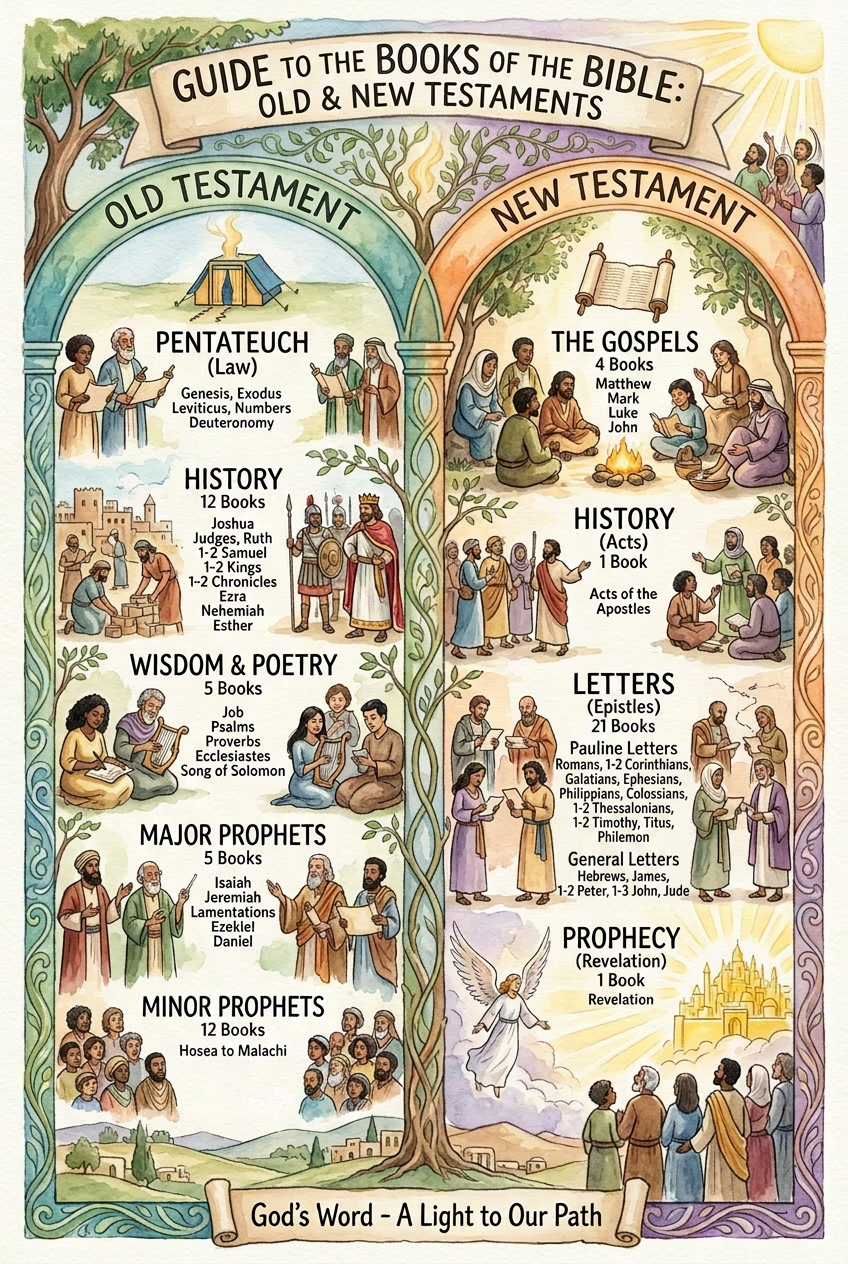
\includegraphics[width=\paperwidth, height=\paperheight]{images/books-of-the-bible.png}
	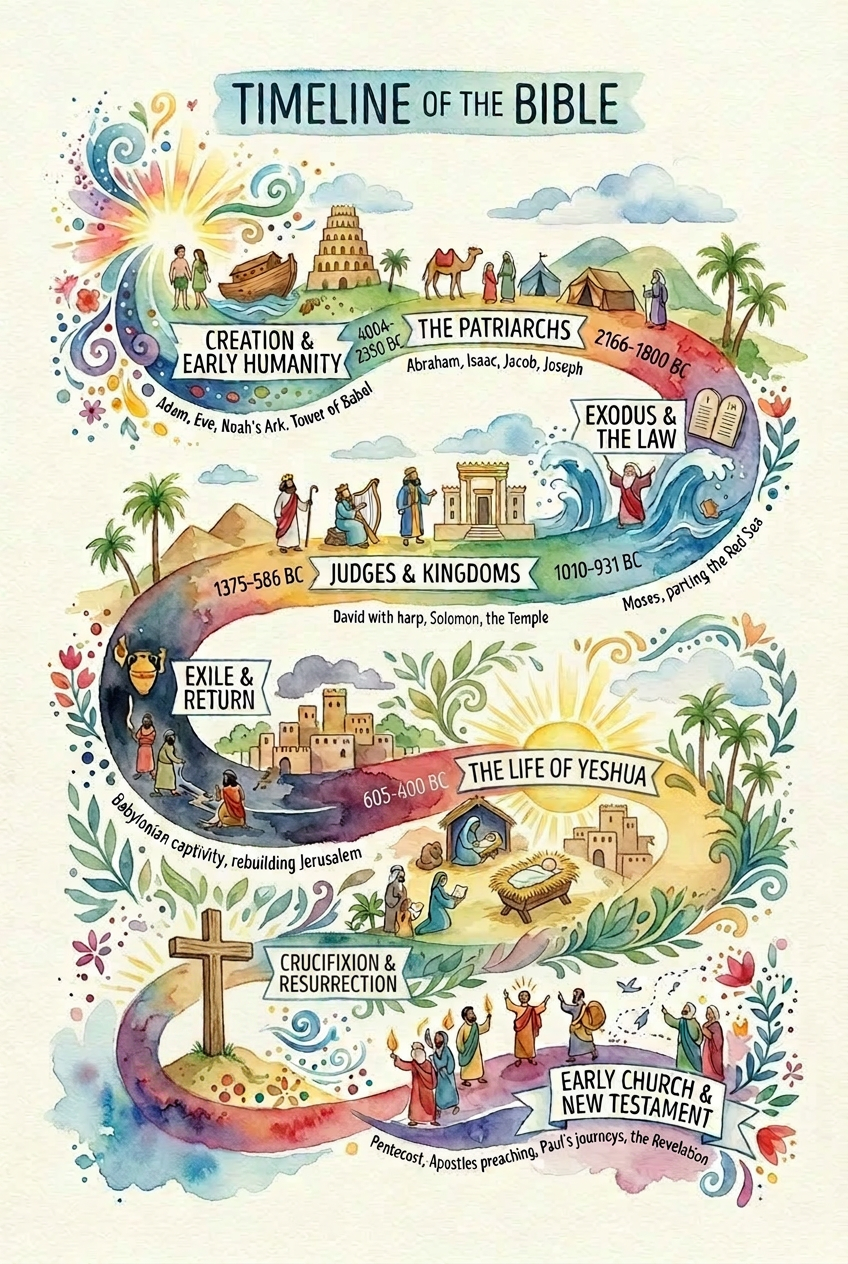
\includegraphics[width=\paperwidth, height=\paperheight]{images/timeline.png}
	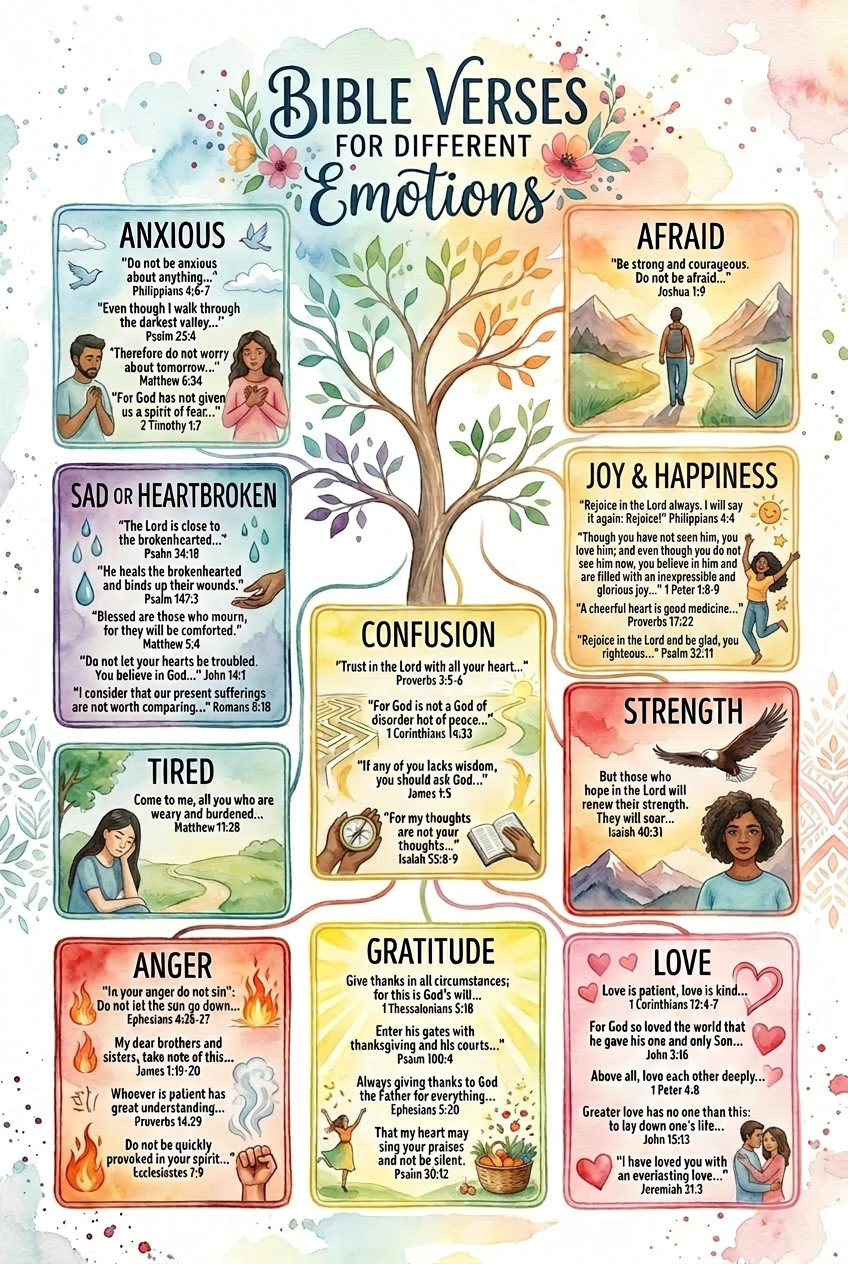
\includegraphics[width=\paperwidth, height=\paperheight]{images/emotions.png}
	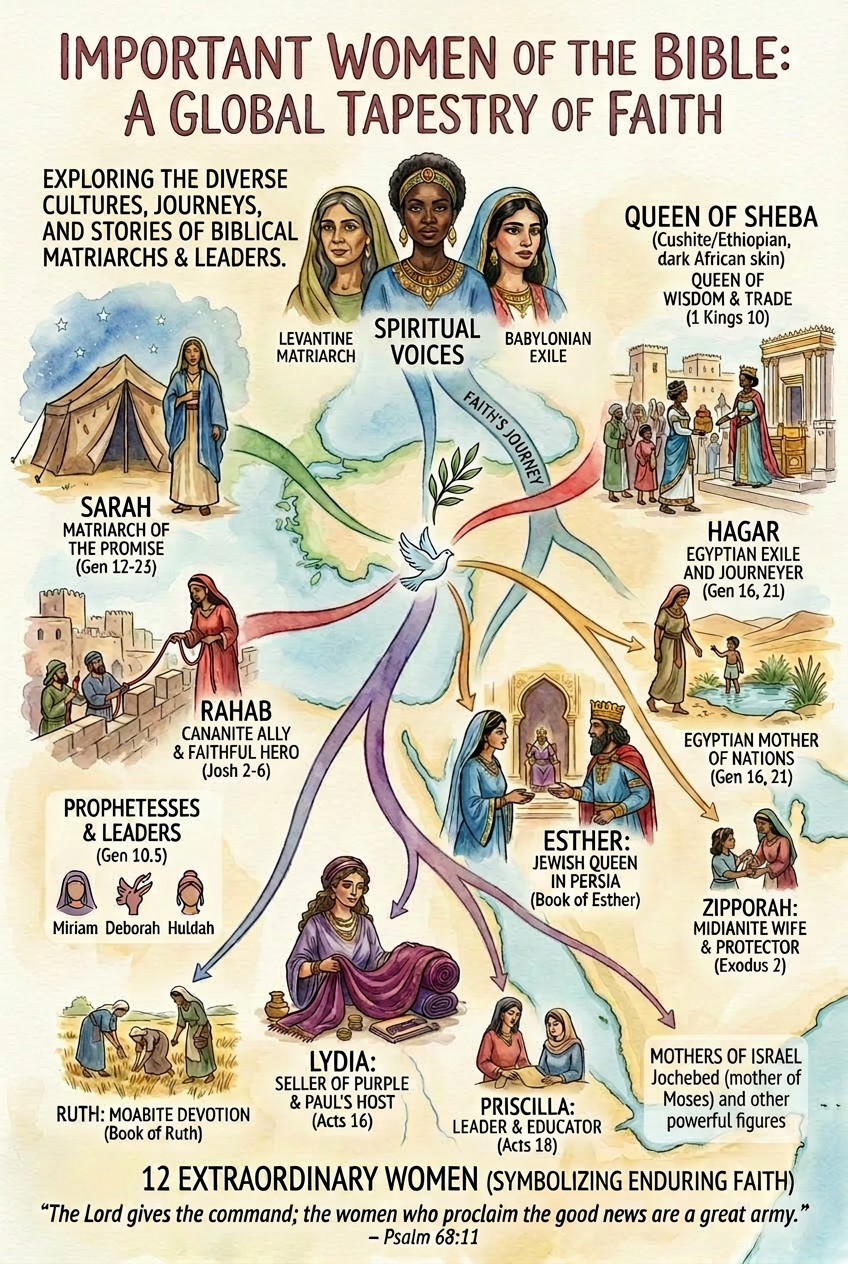
\includegraphics[width=\paperwidth, height=\paperheight]{images/women-of-the-bible.png}
	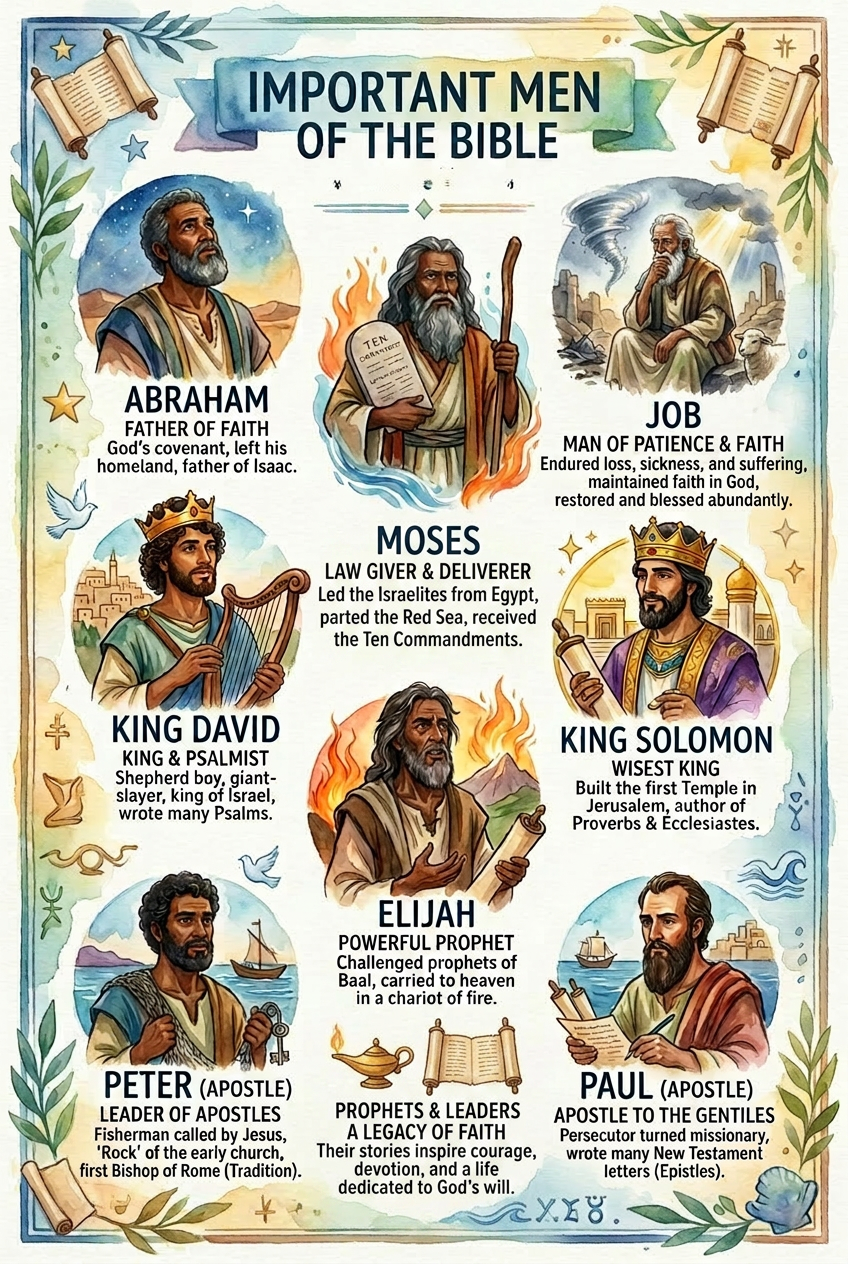
\includegraphics[width=\paperwidth, height=\paperheight]{images/men-of-the-bible.png}
\end{center}
% Restore the document's original margins on the next page
%\clearpage
\restoregeometry
\pagestyle{fancy}
